\chapter{Convolution primer}\label{chap:appendix:conv}
This overview is mainly based on the
paper~\url{https://arxiv.org/pdf/1603.07285.pdf} and the
chapter~\url{https://www.deeplearningbook.org/contents/convnets.html}.

\section{Intro}
Generally, a discrete convolution is a linear transformation that preserves
ordering in the signal (such as width and height axis in images, time axis in
sound clips). The figure below shows an example of a discrete convolution. The
light blue grid is called the \emph{input feature map} (multiple feature maps
are possible, \eg when convoluting the different color channels of an
image). The shaded are is referred to as the \emph{kernel}. The results (in
green) are the \emph{output feature maps}.

\begin{figure}[htpb]
  \centering
  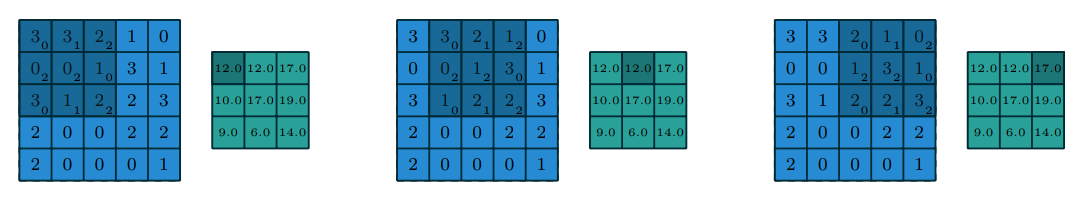
\includegraphics[width=0.8\textwidth]{Figures/discrete_convolution_example}
  \caption{Discrete convolution}%
  \label{fig:conv:ex1}
\end{figure}

The figure is an instance of a 2-D convolution but it can be generalised to N-D
convolutions. The output size $o_j$ of a convolutional layer along an axis $j$
is affected by
\begin{itemize}
\item $i_j$: input size along the axis
\item $k_j$: kernel size along the axis
\item $s_j$: stride along the axis (distance between to consecutive positions of
  the kernel)
\item $p_j$: zero padding along the axis
\end{itemize}
For instance, Figure~\ref{fig:conv:ex2} shows a $3\times 3$ kernel applied to a
$5 \times 5$ input padded with a $1 \times 1$ border of zeros using $2 \times 2$
strides.
\begin{figure}[htpb]
  \centering
  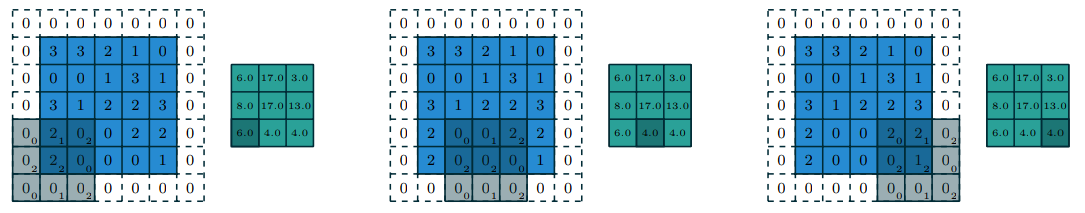
\includegraphics[width=0.8\textwidth]{Figures/discrete_convolution_example2}
  \caption{Different discrete convolution}%
  \label{fig:conv:ex2}
\end{figure}
Note that strides can be interpreted also as follows. Moving the kernel by, \eg,
hops of two is the same thing as moving it by hops of ibe but retaining only odd
output elements.

\subsection*{Pooling}
Another important building block of CNNs are pooling operations. They reduce the
size of feature maps by using some function to summarise subregions, such as
taking the average or the maximum value.

This is done in a sliding window fashion. The content of the window is fed to a
pooling function; so in that sense it is similar to discrete convolution. In discrete
convolution, however, the input gets transformed by forming a linear combination of it whereas in pooling some other function is used.

\section{The Convolution Operation}
In the most general form, convolution is an operation of two functions of a
real-valued argument. Take this example: Suppose we track a spaceship using a
laser sensor that provides a single output $x(t)$, the position of the spaceship
at time $t$, where both $x$ and $t$ are real-valued. Now suppose this sensor is
somewhat noisy. To obtain less noisy estimates of the position, we want to
average over severale measurements. We would like to have a method that weighs
more recent measurements more heavy. To that end, we define a weighting function
$w(a)$, where $a$ is the age of the measurement. If we apply such a weighted
average operation at every moment, we obtain a new function $s$ providing a
smoothed estimate of the position of the spaceship
\begin{equation*}
  s(t) = \int x(a)w(t-a) \da\,.
\end{equation*}
This operation is called \textbf{convolution} and is typically denoted with an
asterisk, \ie $s(t) = (x \ast w)(t)$.

In a machine learning context, the first argument ($x$, in this example) is
usually called the \textbf{input}, and the second argument ($w$) is referred to
as the \textbf{kernel}. The output is called the \textbf{(output) feature map}.

In most of our examples, we will encounter discrete time steps and thus deal
with \emph{discrete convolution}
\begin{equation*}
  s(t) = (x \ast w)(t) = \sum_{a = -\infty}^\infty x(a) w(t - a)\,.
\end{equation*}
The inputs and kernels are tensors that are represented as multi-dimensional
arrays (\eg images $\hat=$ matrices). We assume that only for a finite set of
points are these functions not zero because otherwise they could not be
implemented on a computer with finite storage. The summations then reduce to
summation over a finite number of array elements.

Often, we use convolutions over more than one axis at a time. For example, if
the input is an image $I$ the kernel $K$ will probably also be 2D
\begin{equation*}
  S(i,j) = (I \ast K)(i,j) = \sum_m \sum_n I(m,n)K(i-m, j-n)\,.
\end{equation*}
Since convolution is commutative, we can equivalently write
\begin{equation*}
  S(i,j) = (I \ast K)(i,j) = \sum_m \sum_n I(i-m,j-n)K(m, n)\,,
\end{equation*}
which is often more straightforward to implement. Convolution is commutative
because the kernel is flipped (\ie as $m$ increases the index into the input
increases whereas the index into the kernel decreases). Since the commutative
property is often not an important property in a neural network implementation,
many libraries implement a related function called the
\textbf{cross-correlation} and often call this also convolution
\begin{equation*}
  S(i,j) = (I \ast K)(i,j) = \sum_m \sum_n I(i+m,j+n)K(m, n)\,.
\end{equation*}
Discrete convolution can be viewed as matrix multiplication. For example,
univariate discrete convolutions are equivalent to multiplication by a
\textbf{Toeplitz} matrix (each row is a shifted version of the row above). In
2D, convoltion corresponds to a \textbf{doubly block circulant matrix}. In most
cases, these matrices are sparse.

% In the most general form, convolution is an
% operation of two functions of a real-valued argument. Take this example: Suppose
% we track a spaceship using a laser sensor that provides a single output $x(t)$,
% the position of the spaceship at time $t$, where both $x$ and $t$ are
% real-valued. Now suppose this sensor is somewhat noisy. To obtain less noisy
% estimates of the position, we want to average over severale measurements. We
% would like to have a method that weighs more recent measurements more heavy. To
% that end, we define a weighting function $w(a)$, where $a$ is the age of the
% measurement. If we apply such a weighted average operation at every moment, we
% obtain a new function $s$ providing a smoothed estimate of the position of the
% spaceship
% \begin{equation*}
%   s(t) = \int x(a)w(t-a) \da\,.
% \end{equation*}
% This operation is called \textbf{convolution} and is typically denoted with an
% asterisk, \ie $s(t) = (x \ast w)(t)$.

% In a machine learning context, the first argument ($x$, in this example) is
% usually called the \textbf{input}, and the second argument ($w$) is referred to
% as the \textbf{kernel}. The output is called the \textbf{(output) feature map}.

% In most of our examples, we will encounter discrete time steps and thus deal
% with \emph{discrete convolution}
% \begin{equation*}
%   s(t) = (x \ast w)(t) = \sum_{a = -\infty}^\infty x(a) w(t - a)\,.
% \end{equation*}
% The inputs and kernels are tensors that are represented as multi-dimensional
% arrays (\eg images $\hat=$ matrices). We assume that only for a finite set of
% points are these functions not zero because otherwise they could not be
% implemented on a computer with finite storage. The summations then reduce to
% summation over a finite number of array elements.

% Often, we use convolutions over more than one axis at a time. For example, if
% the input is an image $I$ the kernel $K$ will probably also be 2D
% \begin{equation*}
%   S(i,j) = (I \ast K)(i,j) = \sum_m \sum_n I(m,n)K(i-m, j-n)\,.
% \end{equation*}
% Since convolution is commutative, we can equivalently write
% \begin{equation*}
%   S(i,j) = (I \ast K)(i,j) = \sum_m \sum_n I(i-m,j-n)K(m, n)\,,
% \end{equation*}
% which is often more straightforward to implement. Convolution is commutative
% because the kernel is flipped (\ie as $m$ increases the index into the input
% increases whereas the index into the kernel decreases). Since the commutative
% property is often not an important property in a neural network implementation,
% many libraries implement a related function called the
% \textbf{cross-correlation} and often call this also convolution
% \begin{equation*}
%   S(i,j) = (I \ast K)(i,j) = \sum_m \sum_n I(i+m,j+n)K(m, n)\,.
% \end{equation*}
% Discrete convolution can be viewed as matrix multiplication. For example,
% univariate discrete convolutions are equivalent to multiplication by a
% \textbf{Toeplitz} matrix (each row is a shifted version of the row above). In
% 2D, convoltion corresponds to a \textbf{doubly block circulant matrix}

%%% Local Variables:
%%% mode: latex
%%% TeX-master: "../../main"
%%% End:

